\documentclass[11pt]{article}
\usepackage[T1]{fontenc}
\usepackage[utf8]{inputenc}
\usepackage{lmodern}
\usepackage{amsmath,amssymb,amsthm,mathtools}
\usepackage{microtype}
\usepackage[margin=1.05in]{geometry}
\usepackage{enumitem}
\usepackage{xcolor}
\usepackage{tikz}
\usetikzlibrary{arrows.meta,positioning,fit}
\PassOptionsToPackage{hyphens}{url}
\usepackage{hyperref}
\hypersetup{colorlinks=true,linkcolor=blue!45!black,citecolor=blue!45!black,urlcolor=blue!45!black,pdftitle={An exponential two-way deterministic state lower bound for one-way liveness},pdfauthor={OpenAI}}
\numberwithin{equation}{section}
\newtheorem{theorem}{Theorem}[section]
\newtheorem{lemma}[theorem]{Lemma}
\newtheorem{proposition}[theorem]{Proposition}
\newtheorem{corollary}[theorem]{Corollary}
\theoremstyle{definition}
\newtheorem{definition}[theorem]{Definition}
\theoremstyle{remark}
\newtheorem{remark}[theorem]{Remark}
\newcommand{\D}[1]{\mathcal D_{#1}}
\newcommand{\R}[1]{\mathcal R_{#1}}
\newcommand{\Id}[1]{I_{#1}}
\newcommand{\id}{\mathbf 1}
\DeclareMathOperator{\supp}{supp}
\DeclareMathOperator{\rank}{rank}
\newcommand{\Lfun}{L}
\newcommand{\OWL}{\mathsf{OWL}}
\newcommand{\NFA}{\mathsf{2NFA}}
\newcommand{\DFA}{\mathsf{2DFA}}
\newcommand{\eps}{\varepsilon}
\setlist[enumerate]{itemsep=0.35em,topsep=0.5em}
\setlength{\emergencystretch}{2em}
\allowdisplaybreaks[1]

\title{An exponential two-way deterministic\protect\\state lower bound for one-way liveness}
\author{OpenAI}
\date{September 25, 2026}
\begin{document}
\maketitle
\begin{abstract}
One-way liveness on $h$ points accepts a word of binary relations when
their ordered product is nonempty. For every $h\ge2$, it has a
nondeterministic automaton with $h+3$ states and no left moves, whereas
every equivalent $s$-state two-way deterministic automaton satisfies
$4(s+2)^2\ge2^{\lfloor(h-2)/31\rfloor}$. Partial transition rules, stay
moves, and nonaccepting infinite computations are allowed. The alphabets are
finite and grow with $h$, so the result rules out an alphabet-independent
polynomial state bound for deterministic two-way simulation, already for
one-way nondeterministic sources.
\end{abstract}
\section{Introduction}

Two-way deterministic automata recognize the same languages as one-way
finite automata, as established by Rabin and Scott and by
Shepherdson~\cite{RabinScott1959,Shepherdson1959}. Allowing the head to
return to a symbol can nevertheless change the amount of finite control
needed to recognize a language. How much finite control is needed to
replace nondeterministic choices by deterministic head motion?
Sakoda and Sipser posed the state cost of converting one-way and two-way
nondeterministic finite automata to two-way deterministic automata in
1978~\cite{SakodaSipser1978}.
The question concerns succinctness: the simulator may revisit the input,
but must store all information other than the head position in its finite
state. A polynomial simulation would make nondeterminism inexpensive in
this measure even when the source machine itself moves in both directions.

The witness used here is Sakoda and Sipser's complete family $B_h$,
now called \emph{one-way liveness}: each letter specifies a binary
relation on an $h$-element set, and a word is live when the product of
its letters is nonempty.
Their Theorem~2.3 establishes this family's completeness for
one-way-nondeterministic to two-way-deterministic state
conversion~\cite{SakodaSipser1978}. Our proof below gives the small
source automaton and the context-separation property directly, with
the conventions and exact state counts used here.

Earlier exponential lower bounds restrict the motion of the deterministic
target. Sipser proved an exponential separation for sweeping automata,
whose head changes direction only at an endmarker~\cite{Sipser1980}.
Kapoutsis extended this phenomenon to deterministic machines constrained
to make sublinearly many reversals as a function of input
length~\cite{Kapoutsis2013}. An unrestricted
target can instead reverse at an interior cell and make arbitrarily many
reversals as the input length grows.

Quadratic lower bounds against unrestricted two-way deterministic targets
already occur in Chrobak's work on unary
languages~\cite{Chrobak1986Unary,Chrobak2003Errata}. For the promise restriction of
one-way liveness to words of exactly three relation letters, Kapoutsis
proved the optimal order $\Theta(h^2/\log h)$~\cite{Kapoutsis2018ShortLiveness};
the alphabet there is still the full relation alphabet. Adeogun and
Kapoutsis~\cite{AdeogunKapoutsis2026} prove a quadratic lower bound for
unrestricted deterministic two-way automata against one-way liveness.
We prove an exponential bound for that unrestricted target model.
The source automata use no left moves, whereas the lower bound permits
stay moves, partial transition rules, and nonaccepting infinite
computations in the target.

The main representation difficulty is to account for repeated visits to
a cell while assigning each input symbol a fixed object independent of
its neighbors. We use the Brauer diagram monoid, whose matchings
underlie Brauer's algebras~\cite{Brauer1937,Auinger2012}:
its elements are perfect matchings on two equally sized sets of ports,
and multiplication glues the adjoining sets and contracts paths.
Determinism makes the configurations reaching a designated accepting
sink form a tree. A tour of that tree gives the required matching
representation, with separate leaves for unused transition candidates
ensuring that each cell's wiring depends only on its own symbol.
The algebraic part then proves an exponential lower bound on the number
of ports whenever matching products retain all the information in
arbitrary relation products. All diagram and relation-monoid facts
needed for this argument are proved below.

\subsection{Model and statement}

An automaton has a finite state set and one read-only head on a finite word
over an alphabet $\Sigma$, bracketed by two distinct endmarkers outside
$\Sigma$. Its head starts at the left endmarker in a designated initial
state. A transition changes the state and moves the head left, right, or
not at all; the head cannot cross an endmarker. A transition depends only
on the current state and scanned symbol. Deterministic transition rules
may be partial. A nondeterministic rule permits several successors.
There are no additional heads, writable cells, work tapes, advice, or
randomness. All states, including initial and accepting states, are counted.

Acceptance means that a finite computation reaches an accepting state;
a nonaccepting infinite computation rejects. We initially count an
accepting initial configuration as success. If success instead requires
a positive transition into an accepting state, the normalization in
Section~\ref{sec:machines} uses one additional initial copy. The main
bound below includes this extra state and holds with either convention.

For a finite set $H$, let $\R{H}$ be the monoid of all binary relations
on $H$. Products are in path order from left to right:
\[
 (x,z)\in AB
 \quad\Longleftrightarrow\quad
 \text{there exists }y\in H\text{ with }(x,y)\in A,\ (y,z)\in B.
\]
Write $\Id{F}=\{(x,x):x\in F\}$ for $F\subseteq H$; the identity is
$\Id{H}$ and the zero is the empty relation $0$. For $H=[h]$ define
\begin{equation}
\label{eq:liveness-language}
 \OWL_h=\{R_1\cdots R_\ell\in(\R{[h]})^*:
                  R_1\cdots R_\ell\ne0\}.
\end{equation}
The product of the empty word is $\Id{[h]}$, so $\eps\in\OWL_h$.

\begin{theorem}
\label{thm:main}
For every integer $h\ge2$, the language $\OWL_h$ is recognized by a
nondeterministic automaton with $h+3$ states using no left moves. Every
equivalent deterministic two-way automaton with $s$ states satisfies
\begin{equation}
\label{eq:main-bound}
 4(s+2)^2\ge 2^{\lfloor(h-2)/31\rfloor}.
\end{equation}
If an initially accepting configuration counts as acceptance, $s+2$ in
\eqref{eq:main-bound} may be replaced by $s+1$.
\end{theorem}

\begin{corollary}
\label{cor:no-polynomial}
There are no absolute constants $C,c>0$ such that every $n$-state two-way
nondeterministic automaton over every finite alphabet has an equivalent
two-way deterministic automaton with at most $Cn^c$ states.
\end{corollary}

\begin{proof}
Put $n=h+3$ in Theorem~\ref{thm:main}. Every deterministic equivalent
for this family has at least
\[
 2^{\frac12\lfloor(n-5)/31\rfloor-1}-2
\]
states. This bound exceeds $Cn^c$ for every fixed $C,c$ when $n$ is large
enough. For each $h$ the alphabet has $2^{h^2}$ symbols and is finite.
Since the constants in the proposed simulation must be independent of
the alphabet, the family is within its scope.
\end{proof}

\subsection{Proof architecture}

Write $\D{k}$ for the matching monoid of degree $k$. The proof compares
two bounds on $k$. Theorem~\ref{thm:machine-diagrams} represents each
$s$-state deterministic machine by symbol diagrams in $\D{k}$, with
$k\le4(s+2)^2$. For a machine recognizing $\OWL_h$,
Lemma~\ref{lem:syntactic-quotient} gives a unital surjection from the
submonoid generated by its ordinary-symbol diagrams onto $\R{[h]}$.
Concretely, the map sends each word diagram to its relation product,
preserves multiplication and the empty product, and reaches every
relation on $[h]$. These three properties, including the full image,
are the algebraic input to the lower bound.
Corollary~\ref{cor:divisor-degree} then forces
$k\ge2^{\lfloor(h-2)/31\rfloor}$. These three statements give the deterministic
lower bound in Theorem~\ref{thm:main}.

We prove the algebraic bound first. The \emph{rank} of a matching diagram
counts its pairs joining opposite sides. A diagram $e$ is
\emph{idempotent} if $e^2=e$; its \emph{corner} consists of the diagrams
$z$ with $ez=ze=z$, with identity $e$. Section~\ref{sec:matching} reduces
the corner of an idempotent of rank $r$ to degree $r$, preserving rank
and controlling the indices at which the diagram differs from the
identity. An idempotent of rank $r$ in $\D{k}$ differs
from the identity on at most $2(k-r)$ indices. The support control is
uniform: a family supported in one set remains supported in a single
set of no greater size after reduction. Section~\ref{sec:rank} uses
$32$ conjugates of one idempotent to make $256$ successive relation
additions. A common support set bounds their total rank loss, while
each addition yields a further corner representing all relations on
$h-31$ points. Comparing these bounds doubles the required rank loss
every $31$ points.

Section~\ref{sec:machines} obtains local symbol diagrams by converting
acceptance to reachability of a designated sink. Its undirected component
is a tree, whose doubled tour supplies the matching test. This traversal
has precedents in Sipser's halting method and in the reversible
simulation of Lange, McKenzie, and
Tapp~\cite{SipserHalting1980,LangeMcKenzieTapp2000}. Candidate
transition slots completed by separate leaves make the construction
independent of neighboring symbols. Finally,
Section~\ref{sec:separation} obtains the quotient by using
singleton-identity context letters to test each pair in a relation
product. No input-length or running-time bound is imposed.

\subsection{Related results}

Adeogun and Kapoutsis also analyze limitations of their earlier
lower-bound construction~\cite{AdeogunKapoutsisLimitation2026}. They
prove a quadratic ceiling for its sequences of connectivity properties
and state a general-property extension whose proof is deferred.
The amplification here uses a fixed chain of $256$ additions. Its
exponential bound comes from the inductive lower bound on each rank
loss in a smaller full relation corner, together with one common
support budget for all additions.

The companion paper~\cite[Theorem~1.1]{CompanionComplementation2026}
proves that a nondeterministic two-way automaton for the complement of
$\OWL_h$ requires at least
$\frac12 2^{\lfloor(h-2)/127\rfloor}-1$ states. The present proof
establishes the deterministic bound directly using matching diagrams.
Both results concern state succinctness over
growing alphabets; neither yields a uniform logarithmic-space
separation or a bound measured by transition-table size.

\section{Matching and relation corners}
\label{sec:matching}

We first establish the algebraic properties used in the rank argument.
All monoid products in this paper are in path order: in a product $ab$,
the factor $a$ is placed to the left of the factor $b$.
A homomorphism is called \emph{unital} when it preserves the designated
identities.

\subsection{Matching diagrams, rank, and support}

For an integer $m\geq 0$, let $[m]=\{1,\ldots,m\}$, with
$[0]=\varnothing$.  A \emph{matching diagram of degree $m$} is a perfect
matching on two disjoint sets of ports, a left set and a right set, each
indexed by $[m]$.  Only the paired ports matter; crossings in a drawing
have no significance.  Let $\D{m}$ be the set of these diagrams.

To multiply $a,b\in\D{m}$, identify the right port indexed $i$ of $a$
with the left port indexed $i$ of $b$, for every $i\in[m]$.  In the
resulting finite multigraph, each outside port has degree one and each
identified port has degree two.  Thus every component meeting an outside
port is a path with two outside endpoints.  Pair these endpoints and
discard the components without outside ports.  The result is $ab$.
Parallel edges, when they occur at the interface, are counted separately.

This multiplication is associative.  Indeed, in any string of glued
diagrams, a substring can be replaced by the matching of its boundary
endpoints: each path through the substring is replaced by one edge with
the same endpoints.  This preserves the connections between the outer
ports of the whole string.  Components internal to the substring have
no connection to those ports.  Contracting the first or the last two
factors in a string of three therefore gives the same outside matching.
The diagram $\id_m$ pairing each left port $i$ with right port $i$ is
an identity.  In particular, $\D{0}=\{\id_0\}$ is the one-element
monoid.  The monoids $\D{m}$ are the Brauer diagram
monoids, whose matchings underlie Brauer's
algebras~\cite{Brauer1937}. Their semigroup structure and transversal
rank have been studied in particular by Auinger and by East and
Gray~\cite{Auinger2012,EastGray2017}.

A pair joining opposite sides is a \emph{transversal}; a pair on one
side is a \emph{cap}.  Write $\rank(a)$ for the number of transversals
of $a$, and define
\[
  \supp(a)=\{i\in[m]:
      \text{$a$ does not pair left $i$ with right $i$}\}.
\]
We say that $a$ is \emph{supported in} $J\subseteq[m]$ if
$\supp(a)\subseteq J$.

\begin{lemma}[Rank and support]
\label{lem:rank-basic}
For $a,b\in\D{m}$,
\[
  \rank(ab)\leq \min\{\rank(a),\rank(b)\},
  \qquad
  m-\rank(a)\leq |\supp(a)|.
\]
The units of $\D{m}$ are exactly its rank-$m$ diagrams, which are the
permutation diagrams.  The only rank-$m$ idempotent is $\id_m$.
Conjugation by a permutation diagram preserves rank.
For every $J\subseteq[m]$, the diagrams supported in $J$ form a
submonoid of $\D{m}$.
\end{lemma}

\begin{proof}
Each transversal path in the product uses a transversal of $a$ and a
transversal of $b$.  Different product paths are disjoint, so they use
distinct transversals of either factor.  This proves the rank inequality.
Every index outside $\supp(a)$ supplies a fixed transversal, proving
the support inequality.

A rank-$m$ diagram is a bijection between its two sides and has the
inverse permutation diagram as a two-sided inverse.  Conversely, the
rank inequality forces every unit to have rank $m$.  An idempotent in
a group is its identity, proving the assertion about idempotents.
If $u$ is a permutation diagram, the rank inequality gives
$\rank(uau^{-1})\leq\rank(a)$; applying it to
$a=u^{-1}(uau^{-1})u$ gives the reverse inequality.

If both $a$ and $b$ fix the transversal at an index $i$, their product
also fixes it.  Hence any product of diagrams supported in $J$ is
supported in $J$, and $\id_m$ is supported in every such set.
\end{proof}

\subsection{Reduction at an idempotent}

If $e^2=e$ in a monoid and $S$ is a subset closed under multiplication
and containing $e$, its \emph{corner}
\[
  eSe=\{ese:s\in S\}
\]
is a monoid with identity $e$.  In particular, every $z\in eSe$
satisfies $ez=ze=z$. This is the standard local-monoid construction
of finite-semigroup theory~\cite[Section~2.7]{Pin1997}.
For $m\ge3$, Auinger observes that the corner of the standard
rank-$(m-2)$ projection in $\D{m}$ is isomorphic to
$\D{m-2}$~\cite[Section~3]{Auinger2012}.
The following reduction treats an arbitrary idempotent and realizes its
matching corner on fewer ports. Its third part controls one common support
set for an entire family of sandwiches.

\begin{lemma}[Matching corners]
\label{lem:corners}
Let $e\in\D{m}$ be idempotent and let $r=\rank(e)$.
\begin{enumerate}[label=(\roman*)]
  \item There is a unital injective homomorphism
  \[
    R_e:e\D{m}e\longrightarrow\D{r}
  \]
  satisfying $\rank(R_e(z))=\rank(z)$ for all $z\in e\D{m}e$.
  \item The idempotent satisfies
  \[
    |\supp(e)|\leq 2(m-r).
  \]
  \item For every $J\subseteq[m]$ there is a set $J'\subseteq[r]$,
  depending only on $e$, $J$, and the numbering chosen for $R_e$, such
  that $|J'|\leq |J|$ and
  \[
    \supp(R_e(eae))\subseteq J'
    \quad\text{for every $a\in\D{m}$ supported in $J$}.
  \]
\end{enumerate}
\end{lemma}

\begin{proof}
Let $X,Y\subseteq[m]$ be the indices of the left and right transversal
endpoints of $e$, respectively.  Its transversals define a bijection
$p:X\to Y$, with $|X|=|Y|=r$.

We describe the connector at the interface between two copies of $e$.
Keep two distinct tagged rows of vertices, $R_i$ and $L_i$ for
$i\in[m]$, and put an edge $R_iL_i$ between each matching pair of
indices.  On the $R$ row put the right caps of $e$, and on the $L$ row
put the left caps of $e$.  Thus the degree-one vertices are precisely
\[
  \{R_y:y\in Y\}\ \cup\ \{L_x:x\in X\},
\]
and all other vertices have degree two.  These tagged vertices remain
distinct even when $X$ and $Y$ overlap.  Pairing the endpoints of its
paths, and discarding its closed components, gives a matching on the
$2r$ displayed vertices.

This is exactly the connector encountered by the transversals in
$e\id_m e=e^2$.  Since $\rank(e^2)=r$, all $r$ left transversal
endpoints of the first copy must reach the right boundary of the second.
Consequently the connector cannot pair two $R$ endpoints or two $L$
endpoints: it pairs $R_y$ with $L_{\gamma(y)}$ for a bijection
$\gamma:Y\to X$.  The path from an outer left endpoint $x\in X$
ends at the right endpoint $p(\gamma(p(x)))$.  Equality $e^2=e$ gives
\[
  p(\gamma(p(x)))=p(x),
  \qquad\text{hence}\qquad \gamma(p(x))=x.
\]
Thus $\gamma=p^{-1}$.

Every diagram $z\in e\D{m}e$ contains the left caps of $e$ on its
outer left side and the right caps of $e$ on its outer right side.
Delete precisely these prescribed caps.  The remaining ports are the
left ports indexed by $X$ and the right ports indexed by $Y$, and they
retain a perfect matching.  In particular, any additional caps among
these retained ports remain in the reduced diagram.  Number $X$ by
$[r]$ in any fixed way, and give the right endpoint $p(x)$ the same
number as $x$.  This defines $R_e(z)$.

Figure~\ref{fig:corner-reduction} illustrates the connector and the
numbering for a rank-$2$ idempotent.
\begin{figure}[htbp]
\centering
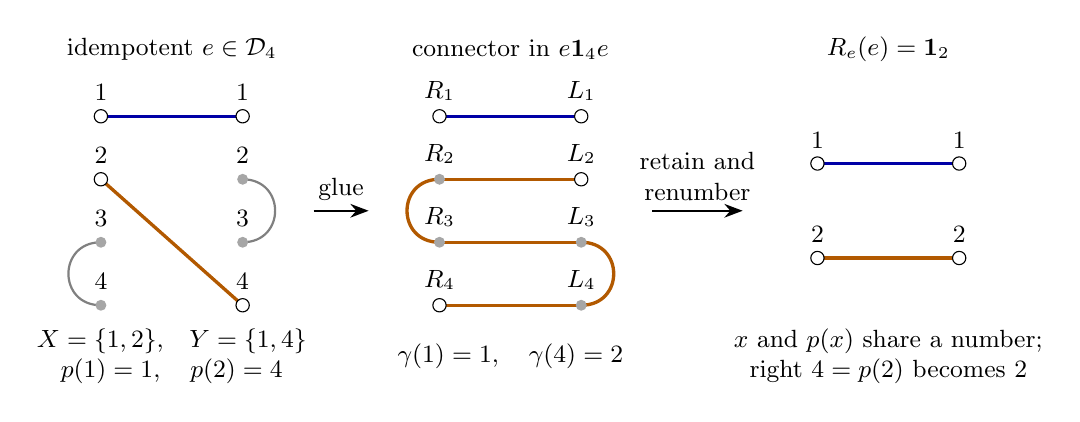
\begin{tikzpicture}[
  >=Stealth,
  every node/.style={font=\small},
  first/.style={very thick,blue!65!black},
  second/.style={very thick,orange!70!black},
  port/.style={circle,fill=gray!70,inner sep=1.4pt},
  retained/.style={circle,draw,fill=white,inner sep=1.7pt}
]
\begin{scope}
\node at (0.9,2.05) {idempotent $e\in\D{4}$};
\foreach \i/\y in {1/1.2,2/0.4,3/-0.4,4/-1.2} {
  \coordinate (eL\i) at (0,\y);
  \coordinate (eR\i) at (1.8,\y);
  \node[anchor=south] at ([yshift=2pt]eL\i) {$\i$};
  \node[anchor=south] at ([yshift=2pt]eR\i) {$\i$};
}
\draw[first] (eL1)--(eR1);
\draw[second] (eL2)--(eR4);
\draw[thick,gray] (eL3) .. controls (-0.55,-0.4) and (-0.55,-1.2) .. (eL4);
\draw[thick,gray] (eR2) .. controls (2.35,0.4) and (2.35,-0.4) .. (eR3);
\foreach \p in {eL3,eL4,eR2,eR3} \node[port] at (\p) {};
\foreach \p in {eL1,eL2,eR1,eR4} \node[retained] at (\p) {};
\node[align=center] at (0.9,-1.85)
  {$X=\{1,2\}$,\quad $Y=\{1,4\}$\\$p(1)=1,\quad p(2)=4$};
\end{scope}

\draw[->,thick] (2.7,0)--node[above] {glue} (3.4,0);

\begin{scope}[shift={(4.3,0)}]
\node at (0.9,2.05) {connector in $e\id_4e$};
\foreach \i/\y in {1/1.2,2/0.4,3/-0.4,4/-1.2} {
  \coordinate (cR\i) at (0,\y);
  \coordinate (cL\i) at (1.8,\y);
  \node[anchor=south] at ([yshift=2pt]cR\i) {$R_{\i}$};
  \node[anchor=south] at ([yshift=2pt]cL\i) {$L_{\i}$};
}
\draw[first] (cR1)--(cL1);
\draw[second] (cR4)--(cL4);
\draw[second] (cL4) .. controls (2.35,-1.2) and (2.35,-0.4) .. (cL3);
\draw[second] (cL3)--(cR3);
\draw[second] (cR3) .. controls (-0.55,-0.4) and (-0.55,0.4) .. (cR2);
\draw[second] (cR2)--(cL2);
\foreach \p in {cR2,cR3,cL3,cL4} \node[port] at (\p) {};
\foreach \p in {cR1,cR4,cL1,cL2} \node[retained] at (\p) {};
\node at (0.9,-1.85) {$\gamma(1)=1,\quad\gamma(4)=2$};
\end{scope}

\draw[->,thick] (7.0,0)--node[above,align=center] {retain and\\renumber} (8.15,0);

\begin{scope}[shift={(9.1,0)}]
\node at (0.9,2.05) {$R_e(e)=\id_2$};
\coordinate (dL1) at (0,0.6);
\coordinate (dL2) at (0,-0.6);
\coordinate (dR1) at (1.8,0.6);
\coordinate (dR2) at (1.8,-0.6);
\draw[first] (dL1)--(dR1);
\draw[second] (dL2)--(dR2);
\foreach \p in {dL1,dL2,dR1,dR2} \node[retained] at (\p) {};
\node[anchor=south] at ([yshift=2pt]dL1) {$1$};
\node[anchor=south] at ([yshift=2pt]dL2) {$2$};
\node[anchor=south] at ([yshift=2pt]dR1) {$1$};
\node[anchor=south] at ([yshift=2pt]dR2) {$2$};
\node[align=center] at (0.9,-1.85)
  {$x$ and $p(x)$ share a number;\\right $4=p(2)$ becomes $2$};
\end{scope}
\end{tikzpicture}
\caption{A rank-$2$ idempotent of degree $4$ and its reduction. In the
left panel, the gray caps are prescribed and the colored transversals
are retained. The connector paths are $R_1$--$L_1$ and
$R_4$--$L_4$--$L_3$--$R_3$--$R_2$--$L_2$, giving
$\gamma=p^{-1}$. Numbering left $x$ and right $p(x)$ alike yields
$R_e(e)=\id_2$. For a general corner element $z$, only the prescribed
outer caps are deleted; every pair among retained ports, including
caps, remains.}
\label{fig:corner-reduction}
\end{figure}


Restoring the prescribed caps and the original indices reconstructs
$z$, so $R_e$ is injective.  Only nontransversal pairs were deleted,
so it preserves rank, and by construction $R_e(e)=\id_r$.
To check multiplication, let $z,w\in e\D{m}e$.  The fixed caps at
their middle interface are the right caps and left caps of $e$.
Their connector is therefore the one just computed: the retained right
port $p(x)$ of $z$ is connected to the retained left port $x$ of $w$.
In the reduced numbering these ports have the same index.
Contracting the connector, including when the reduced diagrams have
caps of their own, thus gives ordinary multiplication in $\D{r}$.
It follows that $R_e(zw)=R_e(z)R_e(w)$, proving (i).

For (ii), suppose that $i\in X\cap Y$.  The vertices $R_i,L_i$ in
the connector have no incident caps, so their edge $R_iL_i$ is an
entire connector path.  Hence $\gamma(i)=i$, and $\gamma=p^{-1}$
implies $p(i)=i$.  Thus every index in $X\cap Y$ is fixed by $e$,
and
\[
  \supp(e)\subseteq([m]\setminus X)\cup([m]\setminus Y).
\]
Both complements have size $m-r$, which proves the bound.

For (iii), consider the full glued graph $e\id_m e$, keeping the
middle identity diagram explicit.  Its transversal paths have the same
outside endpoint pairs as $e$, and so are indexed by the $r$ numbers
used in the reduction.  Mark a transversal path if it uses any middle
identity edge whose index belongs to $J$.  Let $J'$ be the numbers of
the marked paths.  A transversal path may use several middle identity
edges; the only counting fact needed is that different paths are
disjoint.  Each middle identity edge therefore marks at most one
transversal path, and $|J'|\leq|J|$.

Now replace the middle identity by any diagram $a$ supported in $J$.
Every middle identity edge at an index outside $J$ remains present.
An unmarked transversal path used only such edges, so that entire path
survives with the same outside endpoints.  Each of its internal vertices
still has its two original incident edges; a new path cannot attach to
it.  In particular, changes to closed components or to paths with both
endpoints on the same side cannot join an unmarked transversal: all
its middle ports are already paired by the unchanged identity edges.
Its corresponding reduced port is therefore still paired with the
equally indexed port on the other side.  Only numbers in $J'$ can belong
to $\supp(R_e(eae))$.  The construction of $J'$ did not depend on $a$,
as required.

When $r=0$, the prescribed caps exhaust all outside ports.  Then
$eae=e$ for every $a$, and the corner is identified with the singleton
$\D{0}$.  The reduction above is its unique map, and (iii) holds with
$J'=\varnothing$; (ii) also holds since $|\supp(e)|\leq m$.
\end{proof}

The reduction will also be applied to a submonoid $eSe$.  We write
$R_e(eSe)$ for its image in $\D{r}$.  It contains the ambient identity
$\id_r$.  When discussing support in this reduced monoid, the port
set is $[r]$; support in the original monoid still refers to $[m]$.

\subsection{Homomorphic images and permutation lifts}

Every element of a finite semigroup has an idempotent positive power.
Indeed, for an element $x$ there are integers $a\geq1$ and $d\geq1$
such that $x^{k+d}=x^k$ for all $k\geq a$.  Choose $N\geq a$
divisible by $d$.  Then $x^{2N}=x^N$.  If a multiplicative map sends
$x$ to an idempotent $q$, the same is true of every positive power of
$x$, including this idempotent power.

\begin{lemma}[Unit lifts from a minimum-rank corner]
\label{lem:unit-lifts}
Let $S\subseteq\D{m}$ be nonempty and closed under multiplication,
and let $\phi:S\to M$ be an onto multiplicative map to a monoid $M$.
Let $q\in M$ be idempotent.
There is an idempotent $e\in S$ with $\phi(e)=q$.  For every such
$e$, the reduced monoid $R_e(eSe)$ has a unital surjection
\[
  \phi_e:R_e(eSe)\longrightarrow qMq,
  \qquad \phi_e(R_e(z))=\phi(z).
\]
If $e$ has minimum rank among all idempotents in $S$ mapping to $q$,
then every element of $eSe$ mapping to a unit of $qMq$ reduces to a
permutation diagram.  In particular, every unit of $qMq$ has a
permutation lift in $R_e(eSe)$, and that lift is a unit of the reduced
monoid.
\end{lemma}

\begin{proof}
The sets $S$ and $M$ are finite because $\D{m}$ is finite and $\phi$
is onto.  Take any preimage of $q$ and then an idempotent positive power
to obtain $e$.  The image of $eSe$ under $\phi$ is exactly $qMq$:
for any $v\in M$, a preimage $s\in S$ gives
$\phi(ese)=qvq$.  Its identity $e$ maps to the identity $q$ of this
corner.  Lemma~\ref{lem:corners}(i) makes the displayed definition of
$\phi_e$ well-defined and transfers both multiplication and surjectivity.

Suppose now that $e$ has the stated minimum rank, put $r=\rank(e)$,
and let $y\in eSe$ map to a unit $u$ of $qMq$.  The group of units
of $qMq$ is finite, so $u^t=q$ for some positive integer $t$.
Take an idempotent positive power $z$ of $y^t$.  Then $z\in S$ is
idempotent and $\phi(z)=q$.  The rank inequalities and minimum choice
of $e$ give
\[
  r\leq\rank(z)\leq\rank(y)\leq r.
\]
The last inequality uses $y\in eSe$.  Hence $R_e(y)$ has rank $r$
in $\D{r}$ and is a permutation diagram.  Its inverse is a power of
the same finite-order permutation, so lies in $R_e(eSe)$.  Surjectivity
of $\phi_e$ supplies a lift for each unit $u$ and completes the proof.
\end{proof}

\subsection{Corners of the relation monoid}

For a finite set $H$ and a subset $F\subseteq H$, we regard a relation
on $F$ as a relation on $H$ containing no pairs outside $F\times F$.
With $i=\Id{F}$, these are precisely the relations $A$ satisfying
$A=iAi$. Under this identification their monoid is $i\R{H}i$ with
identity $i$. Permutations of a finite set are identified with their
graph relations.

\begin{lemma}[A relation corner]
\label{lem:relation-corner}
Let $P\in\R{H}$ be idempotent, and let $F\subseteq H$ satisfy
$\Id{F}P\Id{F}=\Id{F}$.  Put $i=\Id{F}$ and $Q=PiP$.
Then $Q$ is idempotent, $PQ=QP=Q$, and restriction is a unital
isomorphism
\[
  \theta:Q\R{H}Q\longrightarrow\R{F},
  \qquad \theta(Z)=iZi.
\]
Its inverse sends $A\in\R{F}$ to $PAP=QAQ$.
\end{lemma}

\begin{proof}
The identities $P^2=P$ and $iPi=i$ give
\[
  Q^2=PiP^2iP=P(iPi)P=Q,
  \qquad PQ=QP=Q.
\]
They also give $iQ=iP$, $Qi=Pi$, and $iQi=i$.
If $Z\in Q\R{H}Q$, then $Z=QZQ$ and $PZP=Z$.  Consequently
\[
  Z=PiPZPiP=PiZiP.                         \tag{$*$}
\]
Thus its restriction $iZi$ determines $Z$ uniquely.

Conversely, if $A\in\R{F}$, so that $A=iAi$, then
\[
  QAQ=QiAiQ=PiAiP=PAP,
  \qquad
  i(PAP)i=iPiAiPi=A.
\]
Hence every relation on $F$ is a restriction of an element of the
corner, and $A\mapsto PAP$ is the inverse bijection by~$(*)$.

For multiplication, write $Z=PAP$ and $W=PBP$, where
$A=iZi$ and $B=iWi$ are relations on $F$.  Since $A=Ai$ and
$B=iB$, we have
\[
  ZW=PAP^2BP=PAPBP
     =PA(iPi)BP=PABP.
\]
Restricting this equality gives $\theta(ZW)=AB=\theta(Z)\theta(W)$.
Finally, the identity $Q$ of the source corner restricts to $i$, the
identity of $\R{F}$.  This proves unitality and the claimed isomorphism.
\end{proof}

\section{An exponential rank-loss bound}\label{sec:rank}

We now bound the rank lost by an idempotent diagram whose image adds
one off-diagonal pair to the identity relation. The amplification step
uses $32$ conjugates of that diagram to construct $256$ successive
relation additions. Their joint support bounds the total rank loss,
while a smaller relation corner bounds the loss at each addition.

For every integer $h\ge2$, set
\begin{equation}\label{eq:rank-loss-function}
 \Lfun(h)=2^{\lfloor(h-2)/31\rfloor}.
\end{equation}
All reductions below are the maps $R_e$ of Lemma~\ref{lem:corners}.
Their ranges are regarded as submonoids of the indicated smaller
matching monoids. In particular, their identities are the ambient
identity diagrams, and they preserve absolute rank.

The theorem first assumes permutation lifts in addition to a unital
surjection onto the \emph{entire} relation monoid. A surjection onto only
the relations generated by the displayed additions would not suffice:
the proof must also lift arbitrary elements of smaller relation corners.
Corollary~\ref{cor:divisor-degree} removes the extra lift assumption by
passing to a minimum-rank idempotent corner.

\begin{theorem}[Rank loss for a single relation addition]
\label{thm:rank-loss}
Let $H$ be a finite set of size $h\ge2$, let $m\ge0$, and let
$S\subseteq\D{m}$ be a submonoid containing $\id$.
Suppose that $\phi:S\to\R{H}$ is a unital surjection and that every
permutation of $H$ has a lift in $S$ which is a permutation diagram.
If $a\in S$ is idempotent and
\[
 \phi(a)=\Id{H}\cup\{(x,y)\},\qquad x,y\in H,\quad x\ne y,
\]
then
\[
 m-\rank(a)\ge\Lfun(h).
\]
\end{theorem}

\begin{proof}
We induct on $h$, simultaneously for every ambient degree $m$ and
every choice of $S,\phi,a$ satisfying the hypotheses. Put $t=16$.
For $2\le h<2t+1=33$, one has $\Lfun(h)=1$. A full-rank diagram is
a permutation, and an idempotent permutation is the identity.
Since $\phi$ is unital and $\phi(a)\ne\Id{H}$, the rank of $a$ is
strictly smaller than $m$. This proves the base cases.

Now let $h\ge33$ and assume the theorem for every smaller size at
least two. Write
\[
 c=m-\rank(a).
\]

\paragraph{Conjugates with a common support bound.}
Choose pairwise disjoint sets
\[
 U=\{u_1,\ldots,u_t\},\qquad
 V=\{v_1,\ldots,v_t\},\qquad \{z\}
\]
in $H$. For each ordered pair of distinct points of $H$, a
permutation $\pi$ can send $(x,y)$ to that pair. Choose a
permutation-diagram lift $\widetilde\pi\in S$. Its inverse belongs to
$S$ because a permutation diagram has finite order. In path order,
\[
 \phi(\widetilde\pi^{-1}a\widetilde\pi)
 =\pi^{-1}\bigl(\Id{H}\cup\{(x,y)\}\bigr)\pi
 =\Id{H}\cup\{(\pi(x),\pi(y))\}.
\]
Using the pairs $(u_i,z)$ and $(z,v_j)$ in this construction gives
idempotents $s_i,s'_j\in S$
such that
\begin{equation}\label{eq:rank-conjugate-images}
 \phi(s_i)=\Id{H}\cup\{(u_i,z)\},\qquad
 \phi(s'_j)=\Id{H}\cup\{(z,v_j)\}
 \quad(1\le i,j\le t).
\end{equation}
Conjugation by permutation diagrams preserves rank, so all these
idempotents have rank $m-c$. By Lemma~\ref{lem:corners}(ii), each
has support of size at most $2c$. Thus the set
\[
 J=\bigcup_{i=1}^{t}\supp(s_i)
       \ \cup\ \bigcup_{j=1}^{t}\supp(s'_j)
 \subseteq[m]
\]
has size at most $4tc$. Every product $s_i s'_j$ is supported in $J$,
because diagrams supported in a fixed set form a submonoid.

\paragraph{A chain of $t^2$ additions.}
Put $P_0=\Id{H\setminus\{z\}}$. Choose an idempotent $b_0\in S$
with $\phi(b_0)=P_0$: take any lift of $P_0$ and then a positive
idempotent power. The image stays $P_0$ because $P_0$ is idempotent.
For $1\le i,j\le t$, define
\[
 g_{ij}=b_0s_i s'_j b_0\in b_0Sb_0.
\]
In path order, the two added pairs in
\eqref{eq:rank-conjugate-images} allow the path $u_i,z,v_j$.
The outer factors $P_0$ delete pairs with endpoint $z$, so
\begin{equation}\label{eq:rank-generator-image}
 \phi(g_{ij})=P_0\cup\{(u_i,v_j)\}.
\end{equation}
Figure~\ref{fig:amplification} shows how the same $2t$ conjugates provide
all $t^2$ choices of the pair $(u_i,v_j)$.

\begin{figure}[htbp]
\centering
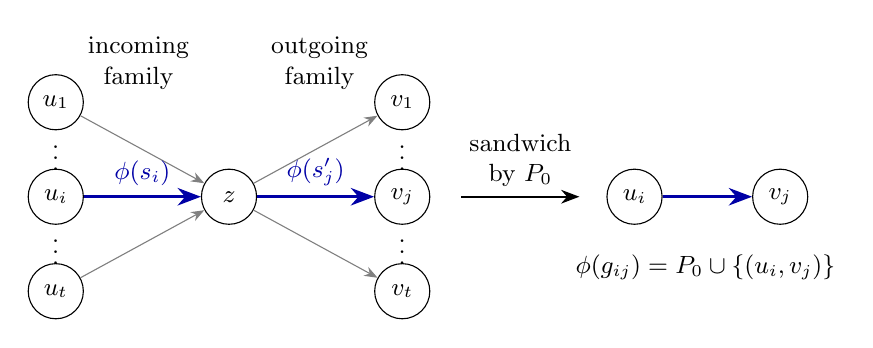
\begin{tikzpicture}[>=Stealth,vertex/.style={circle,draw,minimum size=7mm,inner sep=1pt},every node/.style={font=\small}]
\node[vertex] (upperleft) at (0,1.2) {$u_1$};
\node[vertex] (middleleft) at (0,0) {$u_i$};
\node[vertex] (lowerleft) at (0,-1.2) {$u_t$};
\node at (0,0.6) {$\vdots$};
\node at (0,-0.6) {$\vdots$};
\node[vertex] (hub) at (2.2,0) {$z$};
\node[vertex] (upperright) at (4.4,1.2) {$v_1$};
\node[vertex] (middleright) at (4.4,0) {$v_j$};
\node[vertex] (lowerright) at (4.4,-1.2) {$v_t$};
\node at (4.4,0.6) {$\vdots$};
\node at (4.4,-0.6) {$\vdots$};
\draw[->,gray] (upperleft)--(hub);
\draw[->,very thick,blue!65!black] (middleleft)--node[above] {$\phi(s_i)$} (hub);
\draw[->,gray] (lowerleft)--(hub);
\draw[->,gray] (hub)--(upperright);
\draw[->,very thick,blue!65!black] (hub)--node[above] {$\phi(s'_j)$} (middleright);
\draw[->,gray] (hub)--(lowerright);
\node[align=center] at (1.05,1.7) {incoming\\family};
\node[align=center] at (3.35,1.7) {outgoing\\family};
\draw[->,thick] (5.15,0)--node[above,align=center] {sandwich\\by $P_0$} (6.65,0);
\node[vertex] (retainedleft) at (7.35,0) {$u_i$};
\node[vertex] (retainedright) at (9.2,0) {$v_j$};
\draw[->,very thick,blue!65!black] (retainedleft)--(retainedright);
\node[align=center] at (8.25,-0.9) {$\phi(g_{ij})=P_0\cup\{(u_i,v_j)\}$};
\end{tikzpicture}
\caption{The gray arrows are alternatives from the two families of
relation images; each individual image has one added arrow. The
highlighted path creates the selected pair after both outer factors
delete endpoints at $z$. Identity loops are omitted. Only relations on
$H$ are shown. The common matching support bound comes from taking the
union of the supports of the $32$ conjugates and reducing at $b_0$; the same
conjugates provide all $256$ choices.}
\label{fig:amplification}
\end{figure}


Let $r_0=\rank(b_0)$. Applying Lemma~\ref{lem:corners}(iii) at
$b_0$ to the single set $J$ gives one set $J_0\subseteq[r_0]$,
with $|J_0|\le4tc$, such that
\begin{equation}\label{eq:rank-common-support}
 \supp\bigl(R_{b_0}(g_{ij})\bigr)\subseteq J_0
 \qquad(1\le i,j\le t).
\end{equation}
This set is common to all $t^2$ generators.

List the pairs $(i,j)\in[t]\times[t]$ in any order, without
repetition. Let $E_\ell$ be the set of relation pairs $(u_i,v_j)$
in the first $\ell$ positions, and set
\[
 P_\ell=P_0\cup E_\ell\qquad(0\le\ell\le t^2).
\]
All additional pairs go from $U$ to $V$, and $U\cap V=\varnothing$.
Consequently two additional pairs cannot be composed with each other;
the identity pairs in $P_0$ preserve their endpoints. Thus
\begin{equation}\label{eq:rank-union}
 (P_0\cup A)(P_0\cup B)=P_0\cup(A\cup B)
 \qquad(A,B\subseteq U\times V).
\end{equation}
In particular, $P_\ell^2=P_\ell$.

Starting from $b_0$, construct $b_\ell$ as follows. If $(i,j)$ occupies
position $\ell$, take $b_\ell$ to be a positive idempotent power of
\[
 b_{\ell-1}g_{ij}b_{\ell-1}.
\]
Inductively, its image before taking the power is $P_\ell$, by
\eqref{eq:rank-generator-image} and \eqref{eq:rank-union};
the power has the same image. Hence
\begin{equation}\label{eq:rank-chain}
 b_\ell^2=b_\ell,\qquad
 b_\ell\in b_{\ell-1}Sb_{\ell-1},\qquad
 \phi(b_\ell)=P_\ell.
\end{equation}
Every $b_\ell$ also belongs to $b_0Sb_0$. Indeed, this is true
initially, and this latter set is a submonoid containing every $g_{ij}$;
it is therefore preserved by the construction.

Write
\[
 r_\ell=\rank(b_\ell)\quad(0\le\ell\le t^2),
 \qquad
 \Delta_\ell=r_{\ell-1}-r_\ell\quad(1\le\ell\le t^2).
\]
The nested corners in \eqref{eq:rank-chain} and
Lemma~\ref{lem:rank-basic} give $\Delta_\ell\ge0$.
In the single coordinate system obtained
by reducing at $b_0$, the starting element is the identity and all
generators are supported in $J_0$ by \eqref{eq:rank-common-support}.
The same is true of every constructed product and power, in particular
$R_{b_0}(b_{t^2})$. Rank preservation and the elementary bound of rank
defect by support size give
\begin{equation}\label{eq:rank-total-budget}
 \sum_{\ell=1}^{t^2}\Delta_\ell
 =r_0-r_{t^2}
 \le\bigl|\supp(R_{b_0}(b_{t^2}))\bigr|
 \le|J_0|\le4tc.
\end{equation}

\paragraph{The loss at one addition.}
We claim that for every $1\le\ell\le t^2$,
\begin{equation}\label{eq:rank-single-step}
 2\Delta_\ell\ge\Lfun(h-2t+1).
\end{equation}
Each local argument uses fresh port coordinates to certify this bound
on the already defined absolute rank difference $\Delta_\ell$ in
\eqref{eq:rank-total-budget}.
Fix $\ell$, let $(i,j)$ be its pair, and put
$P=P_{\ell-1}$. Reduce at $b_{\ell-1}$ and define
\[
 T=R_{b_{\ell-1}}(b_{\ell-1}Sb_{\ell-1})
       \subseteq\D{r_{\ell-1}},\qquad
 \beta=R_{b_{\ell-1}}(b_\ell)\in T.
\]
Here $T$ contains the ambient identity
$R_{b_{\ell-1}}(b_{\ell-1})=\id$. The unital-surjection assertion of
Lemma~\ref{lem:unit-lifts} gives
\[
 \theta:T\longrightarrow P\R{H}P,
 \qquad
 \theta(R_{b_{\ell-1}}(w))=\phi(w)
 \quad(w\in b_{\ell-1}Sb_{\ell-1}).
\]
Moreover, $\beta$ is idempotent,
$\theta(\beta)=P_\ell$, and rank preservation gives
\begin{equation}\label{eq:rank-step-support}
 \rank(\beta)=r_\ell,
 \qquad |\supp(\beta)|\le2\Delta_\ell,
\end{equation}
where support now refers to the indices $[r_{\ell-1}]$.

\paragraph{A full relation corner on fewer points.}
Set
\[
 F=\{u_i,v_j\}\cup\bigl(H\setminus(U\cup V\cup\{z\})\bigr),
 \qquad E=\Id{F},\qquad Q=PEP.
\]
Thus $|F|=h-2t+1=h-31$. Among the possible extra pairs in $P$, the
only one with both endpoints in $F$ is $(u_i,v_j)$, which has not yet
been added. Every point of $F$ is different from $z$. Therefore
\[
 EPE=E.
\]
Lemma~\ref{lem:relation-corner} shows that $Q$ is idempotent,
$PQ=QP=Q$, and restriction $Z\mapsto EZE$ is a unital isomorphism
from $Q\R{H}Q$ onto $\R{F}$. In particular,
\[
 Q(P\R{H}P)Q=Q\R{H}Q.
\]
Equation~\eqref{eq:rank-union} also gives $PP_\ell=P_\ell P=P_\ell$.
Since $EQ=EP$ and $QE=PE$, we obtain
\begin{equation}\label{eq:rank-smaller-image}
 E(QP_\ell Q)E
 =EP P_\ell PE
 =EP_\ell E
 =\Id{F}\cup\{(u_i,v_j)\}.
\end{equation}

\paragraph{The second reduction and the induction hypotheses.}
Among the idempotents $d\in T$ with $\theta(d)=Q$, choose one of
minimum rank. Such idempotents exist because $\theta$ is onto and
an idempotent power of a lift of $Q$ still maps to $Q$. This minimum
is taken inside $T$, in its current coordinates in
$\D{r_{\ell-1}}$. Put $r'=\rank(d)$ and reduce once more, defining
\[
 T'=R_d(dTd)\subseteq\D{r'}.
\]
The identity of $T'$ is $R_d(d)=\id$. Its induced map onto
$Q(P\R{H}P)Q$, followed by restriction to $F$, is the unital
surjection
\[
 \psi:T'\longrightarrow\R{F},\qquad
 \psi(R_d(w))=E\theta(w)E\quad(w\in dTd).
\]
By Lemma~\ref{lem:unit-lifts} and the minimum-rank choice of $d$,
every unit of $Q(P\R{H}P)Q$ has a permutation-diagram lift in $T'$.
The restriction isomorphism preserves units, so every permutation of
$F$ has such a lift under $\psi$.

Let $J_\ell=\supp(\beta)\subseteq[r_{\ell-1}]$. Apply
Lemma~\ref{lem:corners}(iii) to the idempotent $d$ in this ambient
matching monoid. There is a set $K\subseteq[r']$ with
$|K|\le|J_\ell|\le2\Delta_\ell$ such that
\[
 \supp\bigl(R_d(d\beta d)\bigr)\subseteq K.
\]
The sandwich $d\beta d$ need not be idempotent. Choose a positive
idempotent power $v$ of its reduction $R_d(d\beta d)$ in $T'$.
Support remains in $K$ under taking powers. By
\eqref{eq:rank-smaller-image}, the image before taking the power is
$\Id{F}\cup\{(u_i,v_j)\}$, an idempotent relation; hence
\[
 v^2=v,
 \qquad \psi(v)=\Id{F}\cup\{(u_i,v_j)\},
 \qquad |\supp(v)|\le2\Delta_\ell.
\]
We have obtained an identity-containing submonoid of $\D{r'}$, a
unital surjection onto $\R{F}$ with permutation lifts, and the
required idempotent above a single off-diagonal addition. These are
all the hypotheses of the theorem at size $|F|=h-31$, which lies
between $2$ and $h-1$. The induction hypothesis and the support bound
therefore give
\[
 \Lfun(h-31)\le r'-\rank(v)
        \le|\supp(v)|\le2\Delta_\ell.
\]
This proves \eqref{eq:rank-single-step} for the chosen $\ell$, and
hence for every step of the chain.

\paragraph{Completion of the recurrence.}
The bounds established above are collected in
Table~\ref{tab:rank-budget}. The support is measured once, in the
coordinates of $b_0$; the separate smaller corners certify each
summand in the resulting rank-loss budget.

\begin{table}[htbp]
\centering
\renewcommand{\arraystretch}{1.22}
\begin{tabular}{lcc}
\hline
Quantity & General expression & $t=16$ \\
\hline
Conjugates & $2t$ & $32$ \\
Successive additions & $t^2$ & $256$ \\
Common support budget & $4tc$ & $64c$ \\
Retained relation points & $h-2t+1$ & $h-31$ \\
Loss per addition & $\frac12\Lfun(h-2t+1)$ & $\frac12\Lfun(h-31)$ \\
Total required loss & $\frac{t^2}{2}\Lfun(h-2t+1)$ & $128\Lfun(h-31)$ \\
\hline
\end{tabular}
\caption{The support upper bound and the inductive rank-loss lower
bound are applied to the same chain. Here $c=m-\rank(a)$.}
\label{tab:rank-budget}
\end{table}

Summing \eqref{eq:rank-single-step} and applying
\eqref{eq:rank-total-budget} yields
\[
 4tc\ge\sum_{\ell=1}^{t^2}\Delta_\ell
      \ge\frac{t^2}{2}\Lfun(h-2t+1).
\]
With $t=16$, it follows that
\[
 c\ge2\Lfun(h-31)
   =2^{1+\lfloor(h-33)/31\rfloor}
   =2^{\lfloor(h-2)/31\rfloor}
   =\Lfun(h).
\]
This completes the induction.
\end{proof}

\begin{corollary}[Degree bound for a unital relation-monoid divisor]
\label{cor:divisor-degree}
Let $H$ be a finite set of size $h\ge2$. If an identity-containing
submonoid $S\subseteq\D{k}$ admits a unital surjection
$\phi:S\to\R{H}$, then
\[
 k\ge\Lfun(h)=2^{\lfloor(h-2)/31\rfloor}.
\]
No hypothesis about permutation lifts is required here.
\end{corollary}

\begin{proof}
Choose an idempotent $e\in S$ of minimum rank among those with
$\phi(e)=\Id{H}$. The set of choices is nonempty, since the identity
of $S$ is one such idempotent. Put $r=\rank(e)$.
By Lemmas~\ref{lem:corners} and~\ref{lem:unit-lifts}, the reduced
corner
\[
 T=R_e(eSe)\subseteq\D{r}
\]
contains the ambient identity and maps unitally onto
$\Id{H}\R{H}\Id{H}=\R{H}$. The minimum-rank choice supplies
permutation-diagram lifts for all permutations of $H$.

Choose distinct $x,y\in H$. Surjectivity supplies a lift in $T$ of
$\Id{H}\cup\{(x,y)\}$. A positive idempotent power of that lift is
an idempotent $a\in T$ with the same image. Theorem~\ref{thm:rank-loss}
applies to this representation, so
\[
 \Lfun(h)\le r-\rank(a)\le r\le k.\qedhere
\]
\end{proof}

\section{Local matching representation of deterministic machines}
\label{sec:machines}

Fix a finite alphabet $\Sigma$.  We use one read-only head on an input
$\vdash w\dashv$, where $w\in\Sigma^*$ and the two endmarkers are
distinct symbols outside $\Sigma$.  A deterministic machine has a finite
state set $Q$, an initial state $q_0$, a set $A\subseteq Q$ of accepting states,
and a partial transition function
\[
 \delta:Q\times(\Sigma\cup\{\vdash,\dashv\})
       \rightharpoonup Q\times\{-1,0,1\}.
\]
The three moves are left, stay, and right.  A transition at an endmarker
never moves beyond that endmarker.  The initial configuration is
$(0,q_0)$, with cell~$0$ carrying $\vdash$.  In this section a computation
accepts when an accepting state occurs at any time, including time~$0$.
A missing transition halts the computation; an infinite computation
without an accepting state rejects.  All states, including initial and
accepting states, count toward $s=|Q|$.

\begin{theorem}[Local matching representation]
\label{thm:machine-diagrams}
For every $s$-state deterministic machine in this model, there is a map
\[
 \eta:\Sigma\cup\{\vdash,\dashv\}\longrightarrow\D{k},
 \qquad k=4(s+1)^2,
\]
with the following property.  Designate ports $1,2$ on each of the two
sides as test ports.  For every word $w=a_1\cdots a_\ell$, the machine
accepts $w$ if and only if the diagram
\[
 \eta(\vdash)\eta(a_1)\cdots\eta(a_\ell)\eta(\dashv)
\]
pairs a left test port with a right test port.  Each symbol diagram is
independent of the input length, the symbol's position, and its
neighboring symbols.

If acceptance instead requires entry into an accepting state after a
positive number of transitions, the same conclusion holds with
$k=4(s+2)^2$.
\end{theorem}

The diagrams will encode a tour of an undirected graph.  Determinism is
used to ensure that the component of one designated vertex is a tree;
no condition is imposed on the other components.
Configuration-tree traversal also underlies Sipser's halting
method~\cite{SipserHalting1980} and the reversible simulation of Lange,
McKenzie, and Tapp~\cite[Section~3.1]{LangeMcKenzieTapp2000}.
We prove the traversal facts needed here and then realize them by
matching diagrams. The candidate-slot construction below supplies
the further requirement that each diagram depend only on the symbol
at its own cell, with the stated quadratic degree.

\subsection{A sink and its tree}

\begin{lemma}[Sink component]
\label{lem:sink-tree}
Let $V$ be finite, let $\sigma:V\rightharpoonup V$ be a partial function,
and let $t\in V$ have no successor.  Make an undirected multigraph on
$V$ with one edge for each defined successor $v\mapsto\sigma(v)$,
retaining self-loops and distinct edges with the same endpoints.
Then a vertex lies in the connected component of $t$ if and only if
some finite sequence of successor steps takes it to $t$.  This
component is a tree.
\end{lemma}

\begin{proof}
Let $B$ be the set of vertices reaching $t$, allowing a sequence of
length zero.  For every successor edge $u\mapsto v$, one has
$u\in B$ if and only if $v\in B$.  One implication prepends that
edge to a path to $t$; the other removes the first step of the unique
successor path from $u$ to $t$.  This removal is legitimate because
$u\ne t$.  Thus membership in $B$ is constant along undirected edges.
Since $t\in B$, its entire component lies in $B$.  Conversely, a
successor path is an undirected path, so every element of $B$ belongs
to that component.

If the component has $v$ vertices, each of its vertices other than
$t$ has exactly one outgoing edge, and $t$ has none.  All these edges
stay in the component, and every edge in the component is counted
once at its source.  Hence the connected multigraph has $v-1$ edges
and is a tree.  In particular, it has neither self-loops nor parallel
edges.
\end{proof}

To apply the lemma, add one new state $f$ to the machine and put
$N=s+1$.  This is an auxiliary successor rule for a reachability
test, not a change in the language to be recognized.  For every
$b\in\Sigma\cup\{\vdash,\dashv\}$, define
\[
 \widehat\delta(q,b)=
 \begin{cases}
  (f,0),&q\in A,\\
  \delta(q,b),&q\in Q\setminus A,\\
  (f,1),&q=f,\ b\ne\dashv,\\
  \text{undefined},&q=f,\ b=\dashv.
 \end{cases}
\]
The first case applies even when the old transition was undefined.
Only the rows at old nonaccepting states retain their old partial
rules, including undefined entries.

For a fixed input of length $\ell$, let
\[
 c_0=(0,q_0),\qquad t=(\ell+1,f).
\]
The original machine accepts precisely when the modified successor
rule reaches $t$ from $c_0$.  Indeed, the computations agree until
the first accepting state, which now leads into $f$ and then to $t$.
Conversely, the first entry into $f$ must come from an old accepting
state.  This also covers acceptance initially or on an endmarker.
Let $G$ be the undirected successor multigraph on all configurations
$(i,q)$, where $0\le i\le\ell+1$ and $q\in Q\cup\{f\}$.
Lemma~\ref{lem:sink-tree} shows that the component of $t$ is a tree,
and that $c_0$ belongs to it exactly on accepted inputs.  Nonaccepting
cycles in other components require no further modification.

\subsection{Tours determined by cyclic orders}

An incidence of an edge at a vertex records its endpoint there.
A loop has two incidences at its vertex.  Choose a cyclic order of
the incidences at every vertex of positive degree.  Regard each edge
as having two directed traversals.  Upon arriving at a vertex along
one incidence, depart along the next incidence in its cyclic order.
At a vertex of degree one this means returning along the same edge.

\begin{lemma}[Tree tour]
\label{lem:tree-tour}
For a finite tree with at least one edge, this rule has a single
cycle on its directed edge traversals, for every choice of cyclic
orders.  If the two joins at two distinct leaves are opened, the
resulting two paths each connect a tip at one leaf to a tip at the
other.
\end{lemma}

\begin{proof}
The rule is a permutation of the directed traversals: a departure
has exactly one preceding arrival, determined by the preceding
incidence in the cyclic order.  A tree consisting of one edge gives
a cycle of its two traversals.

For the induction step, remove a leaf $z$ with neighbor $v$ from
a tree with more than one edge.  Restrict the cyclic order at $v$
by removing the incidence of $vz$.  The smaller tree has one tour
cycle by induction.  Inserting $vz$ back into that order replaces
one transition
\[
 (u,v)\longmapsto(v,w)
\]
of the smaller tour by
\[
 (u,v)\longmapsto(v,z)\longmapsto(z,v)\longmapsto(v,w).
\]
Here $u=w$ is allowed.  No other transition changes.  Thus two new
traversals are inserted into the existing cycle, proving the first
assertion.

Realize the tour as a circular wire, using one lane for each
directed traversal and a join for each arrival-to-departure step.
The joins at two different leaves are two different points on this
circle.  Opening both cuts the circle into two paths, each running
between the two cuts.  Each path consequently has one tip at each
of the two leaves.
\end{proof}

\subsection{Cell diagrams and their composition}

\begin{proof}[Proof of Theorem~\ref{thm:machine-diagrams}]
Use the modified successor rule with its $N=s+1$ states, numbered
by $[N]$.  We first augment its undirected graph by leaves so that
each cell's portion of the graph can be determined from that cell's
symbol alone.

\paragraph{Candidate edges at an internal boundary.}
At every boundary between two neighboring cells, reserve one slot
for each triple
\[
 (d,p,q)\in\{\leftarrow,\rightarrow\}\times[N]\times[N].
\]
The direction $d$ specifies which cell is the prospective source
and which is the prospective target.  The slot represents a
candidate transition from state $p$ in the source cell to state
$q$ in the target cell.  It carries two lane ports, labeled by the
absolute directions of travel $\rightarrow$ and $\leftarrow$.
These labels, together with $(d,p,q)$, give a fixed enumeration of
the
\[
 k=2\cdot N^2\cdot 2=4N^2
\]
ports on either side of a cell.  Equal labels are identified when
neighboring cell diagrams are multiplied.

For each slot put an undirected edge across the boundary.  At its
target end, always attach it to the target cell's state vertex
$q$.  At its source end, attach it to state vertex $p$ if the
modified transition from $p$ on the source cell's symbol is exactly
the transition specified by the slot.  Otherwise attach that end
to a new degree-one vertex in the source cell.  Use a different new
vertex for each unused slot.

Every actual crossing successor edge is represented once, in its
own slot.  Each other slot contributes a single leaf edge attached
to a state vertex.  Keep every actual stay edge inside its cell,
with two distinct incidences when it is a loop.  The resulting
graph is therefore $G$ with additional leaves and leaf edges.
It has the same connectivity between state vertices as $G$, and
the component of $t$ is still a tree.

The target-end attachment makes the construction local: a target
cell does not need to know whether its neighbor uses a slot.
Every possible incoming slot is attached to its indicated state
there.  Only the source cell decides between its state vertex and
a fresh leaf, using its own scanned symbol and successor rule.
Figure~\ref{fig:candidate-slot} isolates this choice for one slot.
\begin{figure}[htbp]
\centering
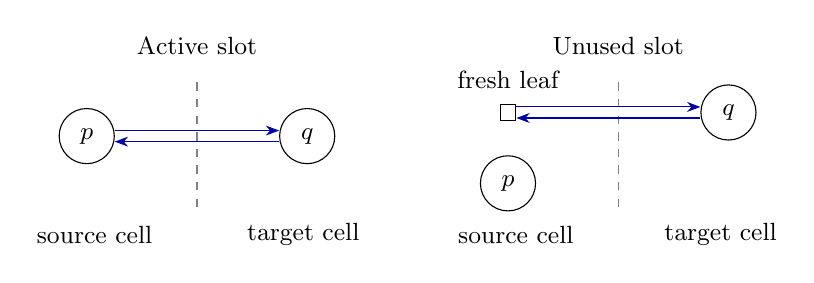
\begin{tikzpicture}[>=Stealth,state/.style={circle,draw,minimum size=7mm,inner sep=1pt},every node/.style={font=\small}]
\node at (1.9,1.15) {Active slot};
\node at (7.25,1.15) {Unused slot};
\draw[dashed,gray] (1.9,-0.9)--(1.9,0.75);
\draw[dashed,gray] (7.25,-0.9)--(7.25,0.75);
\node[state] (activefrom) at (0.5,0) {$p$};
\node[state] (activeto) at (3.3,0) {$q$};
\draw[->,blue!65!black] ([yshift=2pt]activefrom.east)--([yshift=2pt]activeto.west);
\draw[<-,blue!65!black] ([yshift=-2pt]activefrom.east)--([yshift=-2pt]activeto.west);
\node[state] (unusedfrom) at (5.85,-0.6) {$p$};
\node[draw,rectangle,minimum size=2mm,inner sep=0pt] (leaf) at (5.85,0.3) {};
\node[above=2pt of leaf] {fresh leaf};
\node[state] (unusedto) at (8.65,0.3) {$q$};
\draw[->,blue!65!black] ([yshift=2pt]leaf.east)--([yshift=2pt]unusedto.west);
\draw[<-,blue!65!black] ([yshift=-2pt]leaf.east)--([yshift=-2pt]unusedto.west);
\node at (0.6,-1.25) {source cell};
\node at (3.25,-1.25) {target cell};
\node at (5.95,-1.25) {source cell};
\node at (8.55,-1.25) {target cell};
\end{tikzpicture}
\caption{One candidate transition slot with $d=\rightarrow$, with its two travel
lanes. The target end is always attached to state $q$. Only the source
attachment changes: an actual transition uses state $p$, and an unused
slot uses its own new leaf, adding no state-to-state connection.
Thus the target cell needs no information
about the source symbol. Other slots and local cyclic joins are omitted;
lane arrows indicate traversal, not two machine transitions.}
\label{fig:candidate-slot}
\end{figure}


\paragraph{The two outward boundaries.}
An ordinary cell has a neighbor on each side.  The left-marker
cell has only its right neighbor, and the right-marker cell only
its left neighbor.  Use candidate slots exactly on these inward
boundaries.  On the outward side of the left marker, instead
attach a test edge from $c_0$ to a new outer leaf $z_L$.  On the
outward side of the right marker attach a test edge from $t$ to
another new outer leaf $z_R$.

Each test edge has two lanes whose outer tips occupy ports $1,2$
of the corresponding outward side; the same indices serve as ordinary
candidate-lane ports on internal sides.  These tips will remain
unjoined at the outer leaf.  Pair the other outward ports as
$(3,4),(5,6),\ldots,(k-1,k)$, independently of all graph edges.
This uses all remaining ports because $k$ is even.  Denote the
graph including the two test leaves by $\widehat G$.  Its component
containing $t$ is a tree, and its two test leaves are connected if
and only if the machine accepts.

\paragraph{Lanes and local joins.}
Place two travel lanes on every edge of $\widehat G$, one in each
direction of traversal.  Each incidence consequently has an
incoming tip and an outgoing tip.  For an edge with incidences
$i$ and $j$, its lanes connect the outgoing tip at $i$ to the
incoming tip at $j$, and the outgoing tip at $j$ to the incoming
tip at $i$.  This prescription applies also to a loop, whose
incidences are different even though their vertices coincide.

For a crossing edge, each half-lane ends at the corresponding
boundary port.  Absolute travel directions determine the following
local correspondence:
\[
\begin{array}{c|cc}
 \text{side of the cell}&\rightarrow\text{ lane}&\leftarrow\text{ lane}\\
 \hline
 \text{left}&\text{incoming tip}&\text{outgoing tip}\\
 \text{right}&\text{outgoing tip}&\text{incoming tip}
\end{array}
\]
Thus equal-index gluing connects an outgoing half-lane in one
cell to an incoming half-lane in its neighbor, as required.

At every vertex other than $z_L,z_R$, choose a cyclic order of
its incidences and join the incoming tip at each incidence to the
outgoing tip at the next incidence.  A leaf reflects one lane into
the other; a vertex of degree zero requires no joins.  Choose these
orders separately for each symbol type and then use the same orders
at every occurrence of that symbol.  This is possible because all
incidences are local: incoming crossing slots are always present,
outgoing attachments depend only on the scanned symbol, and stay
edges are internal.  Marker incidences, including their test edges,
are likewise fixed by marker type.  Incidences can, for example,
be ordered by their slot labels and their roles in internal edges.

\paragraph{Contracting one cell.}
Inside a cell, every lane tip is incident with one lane and one
local join.  The only exposed ends are its boundary ports, each
used exactly once, including the separately paired outward ports.
Hence the finite wiring inside the cell has degree two at internal
points and degree one at its ports.  Every component containing a
port is a path ending at exactly one other port.  Discard components
without ports and pair the two endpoints of each remaining path.
The result is a perfect matching on the cell's $2k$ ports, hence
an element of $\D{k}$.  Let $\eta(a)$ be this matching for symbol
$a$.

All preceding choices for one cell depend only on $a$, which proves
the asserted symbol locality.  Gluing cells with equal port indices
reconstructs their full wiring.  Contracting paths first within
cells or only after gluing yields the same pairing of outside
ports, by the definition of diagram multiplication.  Consequently
the whole-input diagram in the theorem is precisely the pairing
obtained from the wires of $\widehat G$, with the two test-leaf
joins omitted and the unused outward ports separately paired.
Figure~\ref{fig:tour-test-ports} shows the test-port part of this
contraction in the accepted case.
\begin{figure}[htbp]
\centering
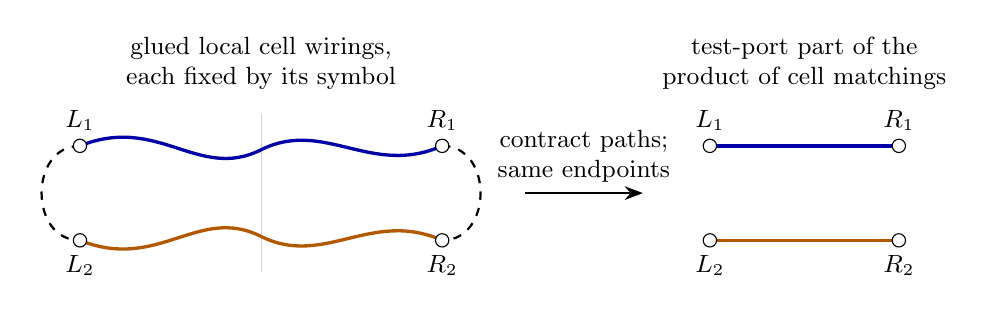
\begin{tikzpicture}[
  >=Stealth,
  every node/.style={font=\small},
  first/.style={very thick,blue!65!black},
  second/.style={very thick,orange!70!black},
  port/.style={circle,draw,fill=white,inner sep=1.7pt}
]
\begin{scope}
\node[align=center] at (2.3,1.65)
  {glued local cell wirings,\\each fixed by its symbol};
\draw[gray!35] (2.3,-1.0)--(2.3,1.0);
\coordinate (wL1) at (0,0.6);
\coordinate (wL2) at (0,-0.6);
\coordinate (wR1) at (4.6,0.6);
\coordinate (wR2) at (4.6,-0.6);
\draw[first] (wL1)
  .. controls (1.0,1.0) and (1.5,0.15) .. (2.3,0.55)
  .. controls (3.1,0.95) and (3.7,0.2) .. (wR1);
\draw[second] (wL2)
  .. controls (1.0,-1.0) and (1.5,-0.15) .. (2.3,-0.55)
  .. controls (3.1,-0.95) and (3.7,-0.2) .. (wR2);
\draw[dashed,thick] (wL1)
  .. controls (-0.65,0.6) and (-0.65,-0.6) .. (wL2);
\draw[dashed,thick] (wR1)
  .. controls (5.25,0.6) and (5.25,-0.6) .. (wR2);
\foreach \p in {wL1,wL2,wR1,wR2} \node[port] at (\p) {};
\node[anchor=south] at ([yshift=2pt]wL1) {$L_1$};
\node[anchor=north] at ([yshift=-2pt]wL2) {$L_2$};
\node[anchor=south] at ([yshift=2pt]wR1) {$R_1$};
\node[anchor=north] at ([yshift=-2pt]wR2) {$R_2$};
\end{scope}

\draw[->,thick] (5.65,0)--node[above,align=center]
  {contract paths;\\same endpoints} (7.15,0);

\begin{scope}[shift={(8.0,0)}]
\node[align=center] at (1.2,1.65)
  {test-port part of the\\product of cell matchings};
\coordinate (mL1) at (0,0.6);
\coordinate (mL2) at (0,-0.6);
\coordinate (mR1) at (2.4,0.6);
\coordinate (mR2) at (2.4,-0.6);
\draw[first] (mL1)--(mR1);
\draw[second] (mL2)--(mR2);
\foreach \p in {mL1,mL2,mR1,mR2} \node[port] at (\p) {};
\node[anchor=south] at ([yshift=2pt]mL1) {$L_1$};
\node[anchor=north] at ([yshift=-2pt]mL2) {$L_2$};
\node[anchor=south] at ([yshift=2pt]mR1) {$R_1$};
\node[anchor=north] at ([yshift=-2pt]mR2) {$R_2$};
\end{scope}
\end{tikzpicture}
\caption{The accepted case, restricted to the four test ports already
exposed on the marker outward sides: $L_i$ and $R_i$ name port $i$ at
the left and right. For the connected sink tree,
Lemma~\ref{lem:tree-tour} shows that restoring the dashed test-leaf
reflections closes one tour cycle; opening them leaves two arcs, each
joining the two sides. Contracting within cells before gluing or after
gluing preserves these outside endpoints and their pairing. The
displayed cross pairing is one possibility. Other ports, caps, and
wire components of the degree-$k$ construction are omitted.}
\label{fig:tour-test-ports}
\end{figure}


\paragraph{Reading acceptance.}
If a wire pairs a left test port to a right test port, it travels
only along edges and joins within one component of $\widehat G$.
The separately paired outward ports are disconnected from these
wires.  Thus $z_L$ and $z_R$ lie in the same component, and the
machine accepts.

Conversely, on an accepted input both test leaves lie in the tree
component containing $t$.  Temporarily add their degree-one
reflection joins.  Lemma~\ref{lem:tree-tour} gives a single circular
wire containing both joins.  Removing them again gives two paths,
each from a left test port to a right test port.  This proves the
acceptance criterion.  Other components, including components with
cycles, cannot affect these paths.

When $w=\eps$, the input still has two distinct adjacent marker
cells.  Their inward sides glue by exactly the same slot scheme,
and both outward test edges are present.  In the connected case the
tree has at least these two edges, so the nonempty-tree hypothesis
of Lemma~\ref{lem:tree-tour} holds.  Thus the argument also gives the
criterion for $\eta(\vdash)\eta(\dashv)$.

Finally, under the positive-transition acceptance convention, first
perform the following operation on the original machine, before the
sink normalization above.  Add a new nonaccepting initial state $q_0'$
with partial row $\delta'(q_0',b)=\delta(q_0,b)$ for every scanned
symbol $b$, using the original partial transition function.
Keep all old states and accepting
states, and leave every transition destination in the old state
set.  Starting at $q_0'$ simulates exactly the original computation
from its first transition onward, so acceptance with the time-zero
convention for this $(s+1)$-state machine is the desired
positive-transition acceptance of the original.  Apply the
construction already proved to obtain degree $4(s+2)^2$.
\end{proof}

Extend $\eta$ to body words by multiplication, with
$\eta(\eps)=\id$.  If $\eta(u)=\eta(v)$, then for every
$x,y\in\Sigma^*$ the whole-input diagrams of $xuy$ and $xvy$
coincide.  The theorem therefore makes $u$ and $v$
indistinguishable in all input contexts, including empty contexts.

\section{From relation products to the state lower bound}
\label{sec:separation}

We now connect the two representations. The use of the full relation
alphabet makes this step elementary: every relation occurs as a single
letter, and two additional letters select any one entry of a product.
This is the context-separation property of one-way
liveness~\cite{AdeogunKapoutsis2026}.

\begin{proposition}
\label{prop:small-nfa}
For $h\ge2$, the language $\OWL_h$ has a nondeterministic automaton with
$h+3$ states, with no left moves.
\end{proposition}

\begin{proof}
Use the $h$ elements of $H=[h]$ as path states, together with three distinct
states $q_{\mathrm{in}},q_{\mathrm{acc}},q_{\mathrm{rej}}$. Start in
$q_{\mathrm{in}}$ on the left endmarker and move right into any path state
$p\in H$. At a letter $R\in\R{H}$ in path state $p$, move right into any
$q$ with $(p,q)\in R$. If there is no such $q$, enter
$q_{\mathrm{rej}}$ by a stay move. At the right endmarker in any path
state, enter $q_{\mathrm{acc}}$ by a stay move. Declare only
$q_{\mathrm{acc}}$ accepting. The rejecting state stays forever, and all
unused rules may enter it by a stay move.

An accepting computation on $R_1\cdots R_\ell$ specifies states
$p_0,\ldots,p_\ell$ with $(p_{j-1},p_j)\in R_j$ for every $j$.
Such states exist exactly when $R_1\cdots R_\ell\ne0$.
For the empty word, the first right move goes directly from the left
marker to the right marker in a path state, and the next step accepts.
This agrees with $\Id{H}\ne0$. All transitions respect the boundaries,
all $h+3$ states are counted, and acceptance always follows a positive
transition.
\end{proof}

\begin{lemma}
\label{lem:syntactic-quotient}
Let $H$ be a nonempty finite set. Suppose a deterministic automaton
recognizing nonzero relation products over $\R{H}$ has a symbol-diagram
representation in $\D{k}$ as in Theorem~\ref{thm:machine-diagrams}.
Let $S\subseteq\D{k}$ be the submonoid generated by the ordinary-symbol
diagrams, including the empty product. Then there is a unital surjection
$S\to\R{H}$ sending each ordinary-symbol diagram to its relation letter.
\end{lemma}

\begin{proof}
For a body word $w$, let $d(w)\in S$ be its diagram product and let
$r(w)\in\R{H}$ be its relation product. Suppose $d(u)=d(v)$. For any
body words $x,y$, associativity gives
\[
 d_{\mathrm L}\,d(x)d(u)d(y)\,d_{\mathrm R}
 =d_{\mathrm L}\,d(x)d(v)d(y)\,d_{\mathrm R},
\]
where $d_{\mathrm L},d_{\mathrm R}$ are the fixed marker diagrams.
The recognition rule therefore gives the same membership decision for
$xuy$ and $xvy$.

If $r(u)\ne r(v)$, choose $(i,j)$ belonging to exactly one of them.
Take $x$ to be the single letter $\Id{\{i\}}$ and $y$ the single letter
$\Id{\{j\}}$. For any relation $A$,
\[
 \Id{\{i\}}A\Id{\{j\}}
 =\begin{cases}
   \{(i,j)\}, & (i,j)\in A,\\
   0, & (i,j)\notin A.
  \end{cases}
\]
Exactly one of the two surrounded words would belong to the language,
a contradiction. Thus $d(u)=d(v)$ implies $r(u)=r(v)$, and
$\phi(d(w))=r(w)$ is well-defined on $S$.

Concatenation proves that $\phi$ preserves multiplication. The empty
word gives $\phi(\id)=\Id{H}$, including when a nonempty word also
has diagram product $\id$. Every relation is the image of its one-letter
diagram, so $\phi$ is surjective.
\end{proof}

\begin{proof}[Proof of Theorem~\ref{thm:main}]
The source-state assertion is Proposition~\ref{prop:small-nfa}.
Let an arbitrary $s$-state deterministic two-way automaton recognize
$\OWL_h$ on all finite words. Under initial-configuration acceptance,
Theorem~\ref{thm:machine-diagrams} gives a representation in
$\D{k}$ with $k=4(s+1)^2$. Lemma~\ref{lem:syntactic-quotient} supplies
a unital surjection from the generated submonoid onto $\R{[h]}$.
Corollary~\ref{cor:divisor-degree} then gives
\[
 4(s+1)^2=k\ge\Lfun(h)=2^{\lfloor(h-2)/31\rfloor}.
\]
With positive-transition acceptance, use the additional initial copy in
Theorem~\ref{thm:machine-diagrams}; its degree is $4(s+2)^2$.
This proves both stated bounds.
\end{proof}

\begin{remark}
The auxiliary vertices and wires used in the matching representation
are an algebraic encoding of a computation graph, not additional memory
granted to the deterministic simulator. The lower bound is proved for
every machine in the ordinary model stated in the introduction. The
family uses a growing finite alphabet, as permitted by the required
alphabet-independent constants; the proof makes no separate
fixed-alphabet claim.
\end{remark}

\bibliographystyle{plainurl}
\begingroup
\raggedright
\bibliography{references}
\endgroup
\end{document}
